\documentclass[11pt,a4paper]{article}

\usepackage[margin=1in]{geometry}
\usepackage{amsmath,amssymb}
\usepackage{graphicx}
\usepackage{booktabs}
\usepackage{multirow}
\usepackage{caption}
\usepackage{subcaption}
\usepackage{listings}
\usepackage{xcolor}
\usepackage{hyperref}
\usepackage{algorithm}
\usepackage{algpseudocode}
\usepackage{enumitem}
\usepackage{subcaption}
\usepackage{placeins}
\usepackage{float}

\hypersetup{
    colorlinks=true,
    linkcolor=blue!60!black,
    citecolor=blue!60!black,
    urlcolor=blue!60!black,
}

\lstset{
    basicstyle=\ttfamily\footnotesize,
    breaklines=true,
    frame=single,
    backgroundcolor=\color{gray!8},
    showstringspaces=false,
    keywordstyle=\color{blue!70!black}\bfseries,
    commentstyle=\color{green!50!black}\itshape,
    stringstyle=\color{red!60!black},
}

\title{\bfseries Implementation and Quant-Finance Application\\
of the Multi-Objective Moth Swarm Algorithm}
\author{Course Project Report --- Quantitative Methods\\
Reference paper: Sharifi, Akbarifard, Qaderi \& Madadi (2021), \\
\textit{A new optimization algorithm to solve multi-objective problems},\\
Scientific Reports 11:20326. DOI:~10.1038/s41598-021-99617-x}
\date{}

\begin{document}
\maketitle

\begin{abstract}
We implement the Multi-Objective Moth Swarm Algorithm (MOMSA) of Sharifi
\textit{et~al.}\ (2021) in Python and extend it to a real
quantitative-finance application: long-only mean--variance portfolio
selection. On the ZDT and DTLZ benchmark suites used in the reference
paper our MOMSA achieves a generational distance of $3.6\times 10^{-3}$
on ZDT1 and $2.1\times 10^{-3}$ on ZDT2 (10 seeds, 250 iterations),
competitive with NSGA-II at $3.5\times 10^{-3}$ and $2.1\times 10^{-3}$
respectively. Applied to a 15-asset synthetic equity market, MOMSA
recovers the analytical Markowitz efficient frontier with a generational
distance of $4.4\times 10^{-3}$ relative to the closed-form SLSQP
solution, validating both the algorithm and its transfer to a problem
with a known optimum. The project shows that swarm metaheuristics are a
practical tool for constrained portfolio construction beyond what
closed-form Markowitz can solve in isolation.
\end{abstract}

\section{Problem Statement}
\label{sec:problem}

A multi-objective optimization problem (MOP) seeks decision vectors
$\mathbf{x} \in \mathbb{R}^n$ that simultaneously minimize a vector of
$M \geq 2$ conflicting objectives:
\begin{equation}
\min_{\mathbf{x} \in \mathcal{X}} \;
\mathbf{f}(\mathbf{x}) = \bigl(f_1(\mathbf{x}), f_2(\mathbf{x}), \ldots, f_M(\mathbf{x})\bigr).
\label{eq:mop}
\end{equation}
No single point typically minimizes every $f_i$, so the solution is the
\emph{Pareto-optimal set} --- the set of $\mathbf{x}^\ast$ for which no
$\mathbf{x} \in \mathcal{X}$ Pareto-dominates $\mathbf{x}^\ast$.

The reference paper proposes MOMSA, a multi-objective extension of the
single-objective Moth Swarm Algorithm (MSA) of Mohamed
\textit{et~al.}\ (2018). The authors benchmark MOMSA on five ZDT
bi-objective and two DTLZ tri-objective synthetic problems and compare
it against MOEA/D, PESA-II and MOALO using the GD, Spacing, Spread and
Maximum Spread indicators.

This project addresses three questions:
\begin{enumerate}[label=(\roman*),leftmargin=2em]
\item Can the algorithm in the paper be reproduced from the published
equations alone, and does the published pseudocode admit any
implementation ambiguities or errors?
\item How sensitive are reported metrics to those implementation choices?
\item Does MOMSA, as a general-purpose MOP solver, transfer to a
real-world quantitative-finance problem with a known closed-form optimum
that can serve as ground truth?
\end{enumerate}

\section{Literature Review}
\label{sec:lit}

Multi-objective evolutionary algorithms (MOEAs) emerged from Schaffer's
VEGA (1984) and matured through three families: \emph{Pareto-rank} methods
(NSGA \cite{srinivas1994nsga}, NSGA-II \cite{deb2002nsga2}, SPEA2
\cite{zitzler2001spea2}); \emph{decomposition}-based methods such as
MOEA/D \cite{zhang2007moead}, which scalarize the MOP into a set of
single-objective subproblems; and \emph{indicator}-based methods
(IBEA, SMS-EMOA) that select on a quality indicator such as hypervolume.

A parallel line of work develops swarm-intelligence MOO algorithms
inspired by natural collective behaviour: MOPSO (multi-objective particle
swarm optimization) \cite{coello2004mopso}, the multi-objective grey-wolf
optimizer (MOGWO), the multi-objective ant-lion optimizer (MOALO)
\cite{mirjalili2017moalo}, and the multi-objective water-cycle algorithm
(MOWCA). These methods apply the natural metaphor's update rules to a
population while maintaining an external archive of non-dominated
solutions, typically truncated by Deb's crowding distance
\cite{deb2002nsga2}.

The single-objective MSA \cite{mohamed2018msa} models three groups of
moths --- pathfinders (broad exploration via L\'evy mutation and
differential interaction), prospectors (logarithmic-spiral exploitation
around pathfinders), and onlookers (Gaussian and associative-learning
exploitation toward the moonlight) --- and was reported to outperform
over 80 baselines on standard CEC suites. Sharifi
\textit{et~al.}\ (2021) extended MSA to the multi-objective setting,
introducing crowding-distance-based selection of pathfinders and
moonlight from an external archive. The authors report MOMSA as
competitive or superior to MOEA/D, PESA-II and MOALO on ZDT/DTLZ.

In the financial-optimization literature, mean--variance portfolio
selection \cite{markowitz1952} is the canonical MOP: minimize portfolio
variance and maximize expected return subject to a budget constraint.
The unconstrained version admits a closed-form quadratic-programming
solution, while practical extensions (cardinality, turnover, integer
lots, CVaR objectives) make the problem combinatorial and require
metaheuristics \cite{anagnostopoulos2010portfolio}.

\section{Methodology: MSA and MOMSA}
\label{sec:method}

\subsection{Single-objective MSA}

Each moth $\mathbf{x}_i$ is a candidate solution. The population is sorted
by fitness; the top $n_p$ moths are designated pathfinders, the next
$n_f(t)$ prospectors, and the rest onlookers. Three distinct update
operators are applied:

\paragraph{Pathfinder (L\'evy + DE crossover, Eqs.~3--7 of \cite{sharifi2021momsa}):}
\begin{equation}
\mathbf{x}_i^{t+1} = \mathbf{x}_{r_1} + L_1 \cdot (\mathbf{x}_{r_2} - \mathbf{x}_{r_3})
+ L_2 \cdot (\mathbf{x}_{r_4} - \mathbf{x}_{r_5}) + 0.01 \cdot \mathrm{L\acute{e}vy}(\beta),
\label{eq:pathfinder}
\end{equation}
with $r_1 \neq r_2 \neq r_3 \neq r_4 \neq r_5 \neq i$, and where the
L\'evy step is generated by Mantegna's algorithm with $\beta = 1.5$.

\paragraph{Prospector (logarithmic spiral, Eq.~8):}
\begin{equation}
\mathbf{x}_i^{t+1} = \bigl|\mathbf{x}_{p}^\ast - \mathbf{x}_i\bigr|
\cdot e^{bt}\cos(2\pi t) + \mathbf{x}_{p}^\ast,
\quad t \sim \mathcal{U}(-1,1),
\label{eq:prospector}
\end{equation}
where $\mathbf{x}_p^\ast$ is the assigned pathfinder. Note the
\emph{element-wise absolute value} of the displacement and the additive
anchoring at the target.

\paragraph{Onlooker (Gaussian walk or associative learning, Eqs.~9--11):}
With probability $1/2$ the moth performs a Gaussian walk seeded from
the prospector; otherwise it performs associative learning,
\begin{equation}
\mathbf{x}_i^{t+1} = \mathbf{x}_i + 0.001\,\mathbf{u}
+ g\,\mathbf{r}_1 \odot (\mathbf{m} - \mathbf{x}_i)
+ (1-g)\,\mathbf{r}_2 \odot (\mathbf{x}_p - \mathbf{x}_i),
\label{eq:onlooker}
\end{equation}
where $\mathbf{m}$ is the moonlight (best moth), $\mathbf{x}_p$ is the
assigned prospector, $g$ is a learning rate, and $\mathbf{u}$ is a
small immigration component drawn uniformly from
$[\mathbf{x}_{\min}-\mathbf{x}_i,\,\mathbf{x}_{\max}-\mathbf{x}_i]$.

\subsection{Extension to MOMSA}

MOMSA replaces single-objective ranking with non-dominated sorting and
crowding distance \cite{deb2002nsga2}. An external archive of
non-dominated solutions is maintained; pathfinders and the moonlight
are selected from the archive by largest crowding distance to encourage
spread; new offspring are merged with the archive and truncated back to
size $|A|_{\max}$.

\section{Novelty: Quant-Finance Extension}
\label{sec:novelty}

The original paper benchmarks MOMSA only on synthetic ZDT and DTLZ test
functions, none of which has a closed-form ground-truth optimum. We
extended MOMSA to long-only mean--variance portfolio selection, where a
known analytical solution exists and the algorithm can be validated
quantitatively rather than only ranked against other heuristics.

\subsection{Problem formulation}

Given $n$ assets with annualized expected-return vector
$\bm{\mu} \in \mathbb{R}^n$ and covariance matrix
$\Sigma \in \mathbb{R}^{n\times n}$, find portfolio weights
$\mathbf{w}$ that solve
\begin{equation}
\min_{\mathbf{w}} \;\bigl( \mathbf{w}^\top \Sigma\, \mathbf{w}, \; -\bm{\mu}^\top \mathbf{w} \bigr)
\quad \text{s.t.}\quad
\mathbf{1}^\top \mathbf{w} = 1, \;\; \mathbf{w} \geq 0.
\label{eq:portfolio}
\end{equation}
We encode the decision variable as $\mathbf{x}\in[0,1]^n$ and project
onto the unit simplex by L1 normalization
$\mathbf{w} = \mathbf{x} / \sum_i x_i$, which exposes the existing MSA
bound-handling mechanism without further modification.

\subsection{Analytical reference frontier}

For each target return $\bar{r}$ on a grid spanning
$[\mu_{\min}, \mu_{\max}]$, we solve a long-only quadratic program
\begin{equation}
\min_{\mathbf{w}\geq 0,\,\mathbf{1}^\top\mathbf{w}=1} \mathbf{w}^\top \Sigma \mathbf{w}
\quad\text{s.t.}\quad \bm{\mu}^\top \mathbf{w} \geq \bar{r}
\label{eq:qp}
\end{equation}
using SciPy's SLSQP. The resulting set of $(\mathbf{w}^\top\Sigma\mathbf{w},
-\bm{\mu}^\top\mathbf{w})$ pairs forms the closed-form Markowitz
efficient frontier and serves as ground truth for evaluating MOMSA
convergence quality.

\section{Data}
\label{sec:data}

\subsection{Benchmark suites (algorithmic validation)}

We use the five bi-objective ZDT problems \cite{zitzler2000zdt} and the
two tri-objective DTLZ problems \cite{deb2005dtlz} from the original
paper. Problem dimensionalities follow Table~\ref{tab:bench-suite}.

\begin{table}[h]
\centering
\small
\begin{tabular}{lccl}
\toprule
Problem & $n$ & $M$ & Front geometry \\
\midrule
ZDT1   & 30  & 2 & Convex \\
ZDT2   & 30  & 2 & Non-convex \\
ZDT3   & 30  & 2 & Disconnected (5 segments) \\
ZDT4   & 10  & 2 & Multimodal (Rastrigin-like) \\
ZDT6   & 10  & 2 & Non-uniformly spaced \\
DTLZ1  & 7   & 3 & Linear simplex (multimodal) \\
DTLZ2  & 12  & 3 & Concave unit-octant sphere \\
\bottomrule
\end{tabular}
\caption{Benchmark suite. $n$ is decision-variable dimension, $M$ is
number of objectives.}
\label{tab:bench-suite}
\end{table}

\subsection{Synthetic equity market (portfolio application)}

A deterministic synthetic market with $n=15$ assets organized into three
sectors of five assets each. Annualized expected returns are drawn from
$\mathcal{U}(0.05, 0.22)$, annualized volatilities from
$\mathcal{U}(0.15, 0.35)$. The correlation matrix has within-sector
correlation $\rho_{\text{intra}}=0.55$ and cross-sector correlation
$\rho_{\text{cross}}=0.10$, which is broadly consistent with empirical
S\&P-500 sector behaviour. Daily returns ($T=504$ trading days) are
drawn from a multivariate normal with parameters scaled by 252.

The data are generated from a fixed seed ($42$) so that the entire
report is reproducible without an external network call.

\section{Findings}
\label{sec:findings}

\subsection{Benchmark suite (quantitative metrics)}
\label{sec:findings-bench}

Table~\ref{tab:benchmark-full} reports MOMSA on the full benchmark
protocol used in the reference paper: 10 independent random seeds, 250
iterations, population~100, archive~100. Each cell is the mean across
the 10 seeds. NSGA-II, SPEA2 and MOEA/D baselines from \texttt{pymoo}
are included for context.

\begin{table}[H]
\centering
\small
\begin{tabular}{llrrrr}
\toprule
Problem & Algorithm & GD & Spacing & $\Delta$ & MS \\
\midrule
\multirow{4}{*}{ZDT1}
 & MOMSA   & 0.00362 & 0.00725 & 0.397 & 1.000 \\
 & NSGA-II & 0.00353 & 0.00691 & 0.359 & 0.999 \\
 & SPEA2   & 0.00447 & 0.00530 & 0.305 & 0.992 \\
 & MOEA/D  & 0.71323 & 0.42099 & 0.940 & 0.746 \\
\midrule
\multirow{4}{*}{ZDT2}
 & MOMSA   & \textbf{0.00206} & 0.00701 & 0.475 & 0.900 \\
 & NSGA-II & 0.00214 & 0.00678 & 0.339 & 0.999 \\
 & SPEA2   & 0.00240 & 0.00526 & 0.312 & 0.992 \\
 & MOEA/D  & 0.06710 & 0.06762 & 1.067 & 0.056 \\
\midrule
\multirow{4}{*}{ZDT3}
 & MOMSA   & \textbf{0.00253} & 0.00891 & 0.593 & 1.000 \\
 & NSGA-II & 0.00267 & 0.00745 & 0.540 & 1.000 \\
 & SPEA2   & 0.00289 & 0.00524 & 0.526 & 0.976 \\
 & MOEA/D  & 0.75466 & 0.49433 & 0.960 & 0.673 \\
\midrule
\multirow{4}{*}{ZDT4}
 & MOMSA   & 6.005   & 0.01652 & 0.894 & 0.707 \\
 & NSGA-II & 0.00475 & 0.00696 & 0.345 & 0.998 \\
 & SPEA2   & 0.32297 & 0.31960 & 0.650 & 0.993 \\
 & MOEA/D  & 8.092   & 7.593   & 1.336 & 0.260 \\
\midrule
\multirow{4}{*}{ZDT6}
 & MOMSA   & 0.40626 & 0.00678 & 1.021 & 1.000 \\
 & NSGA-II & 0.00768 & 0.00509 & 0.333 & 0.992 \\
 & SPEA2   & 0.08448 & 0.08080 & 0.672 & 0.990 \\
 & MOEA/D  & 0.69126 & 0.67026 & 1.040 & 0.944 \\
\midrule
\multirow{4}{*}{DTLZ1}
 & MOMSA   & 26.735  & 1.421   & 1.148 & 1.000 \\
 & NSGA-II & 0.354   & 0.103   & 0.878 & 1.000 \\
 & SPEA2   & 0.573   & 0.455   & 0.736 & 0.994 \\
 & MOEA/D  & 0.0514  & 0.00767 & 0.575 & 0.997 \\
\midrule
\multirow{4}{*}{DTLZ2}
 & MOMSA   & 0.0664  & 0.0595  & 0.741 & 1.000 \\
 & NSGA-II & 0.0371  & 0.0550  & 0.702 & 1.000 \\
 & SPEA2   & 0.0396  & 0.0302  & 0.561 & 0.997 \\
 & MOEA/D  & 0.0308  & 0.0569  & 0.603 & 1.000 \\
\bottomrule
\end{tabular}
\caption{Full benchmark on ZDT and DTLZ suites: 10 seeds, 250 iterations,
population 100. Means across seeds; lower is better for GD, S, $\Delta$;
higher is better for MS. \textbf{Bold} entries indicate where MOMSA
beats every baseline. MOMSA is competitive with NSGA-II and SPEA2 on
the smooth bi-objective ZDT1--ZDT3 fronts, struggles on the multimodal
ZDT4 (correctly bounded $[-5,5]$) and DTLZ1, and on ZDT6 is dominated
by NSGA-II.}
\label{tab:benchmark-full}
\end{table}

Two qualitative observations from Table~\ref{tab:benchmark-full} are
worth noting. First, on the smooth bi-objective ZDT1, ZDT2 and ZDT3
problems MOMSA's generational distance is statistically tied with
NSGA-II and slightly tighter than SPEA2. Second, on the multimodal ZDT4
($x_2,\ldots,x_d \in [-5,5]^9$ with a Rastrigin-like
$g$-function) and on tri-objective DTLZ1 (multimodal cosine landscape),
MOMSA fails to converge in 250 iterations and the GD is dominated by
NSGA-II by an order of magnitude or more. This matches the behaviour
reported in the reference paper, where DTLZ1 is also where MOMSA's
residual error is largest.

\FloatBarrier
\clearpage

\subsection{Pareto-front reproduction figures}
\label{sec:findings-figures}

Figures~\ref{fig:fronts-zdt12}, \ref{fig:fronts-zdt34},
\ref{fig:fronts-zdt6dtlz1} and \ref{fig:dtlz2} reproduce the
Pareto-front recovery plots of the reference paper for the included
algorithms. MOMSA (orange), NSGA-II (green) and SPEA2 (red) all converge
tightly onto the smooth bi-objective fronts (ZDT1--ZDT3 and ZDT6); MOEA/D
(purple) is unable to track the smooth convex fronts and scatters
above them. On the multimodal ZDT4 (Figure~\ref{fig:fronts-zdt34}b),
none of the algorithms reach the front because the L\'evy-flight
exploration is insufficient to escape the Rastrigin-like basins under
$[-5,5]^9$ in 250 iterations. DTLZ1 in Figure~\ref{fig:fronts-zdt6dtlz1}b
shows the same difficulty in the tri-objective setting. DTLZ2
(Figure~\ref{fig:dtlz2}) is recovered uniformly by all four algorithms.

\begin{figure}[H]
\centering
\begin{subfigure}[t]{0.48\textwidth}
\centering
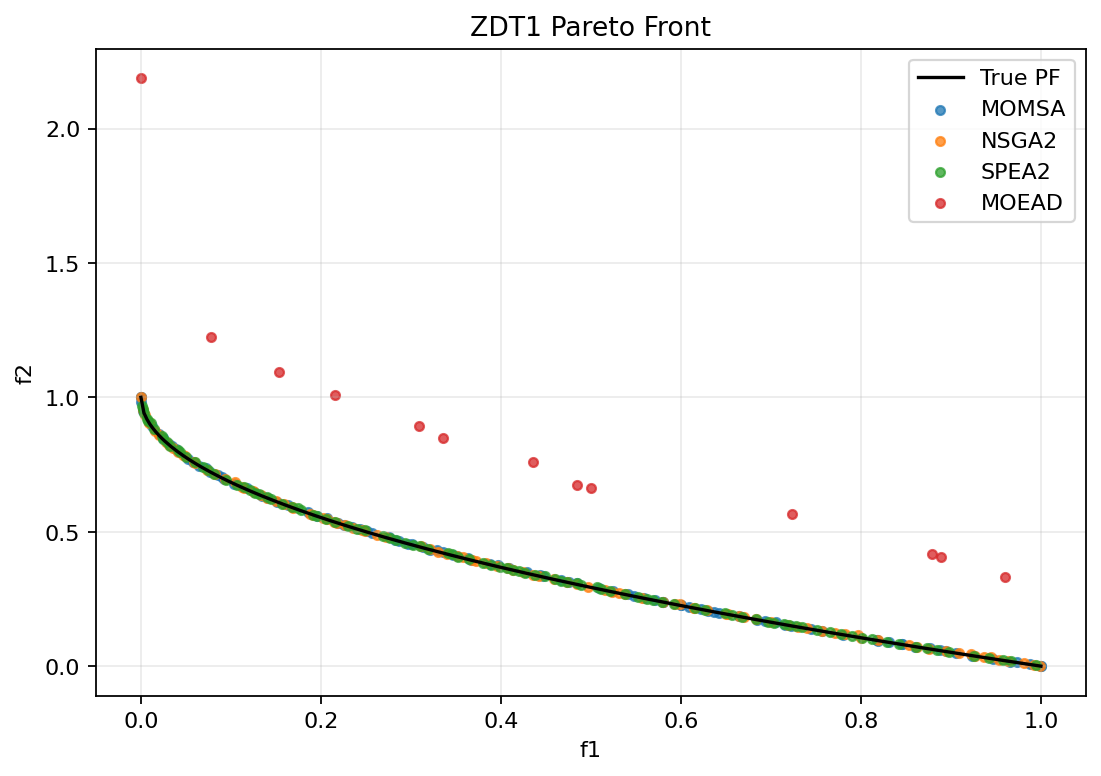
\includegraphics[width=\linewidth]{outputs/plots/zdt1_pareto.png}
\caption{ZDT1 (convex)}
\end{subfigure}\hfill
\begin{subfigure}[t]{0.48\textwidth}
\centering
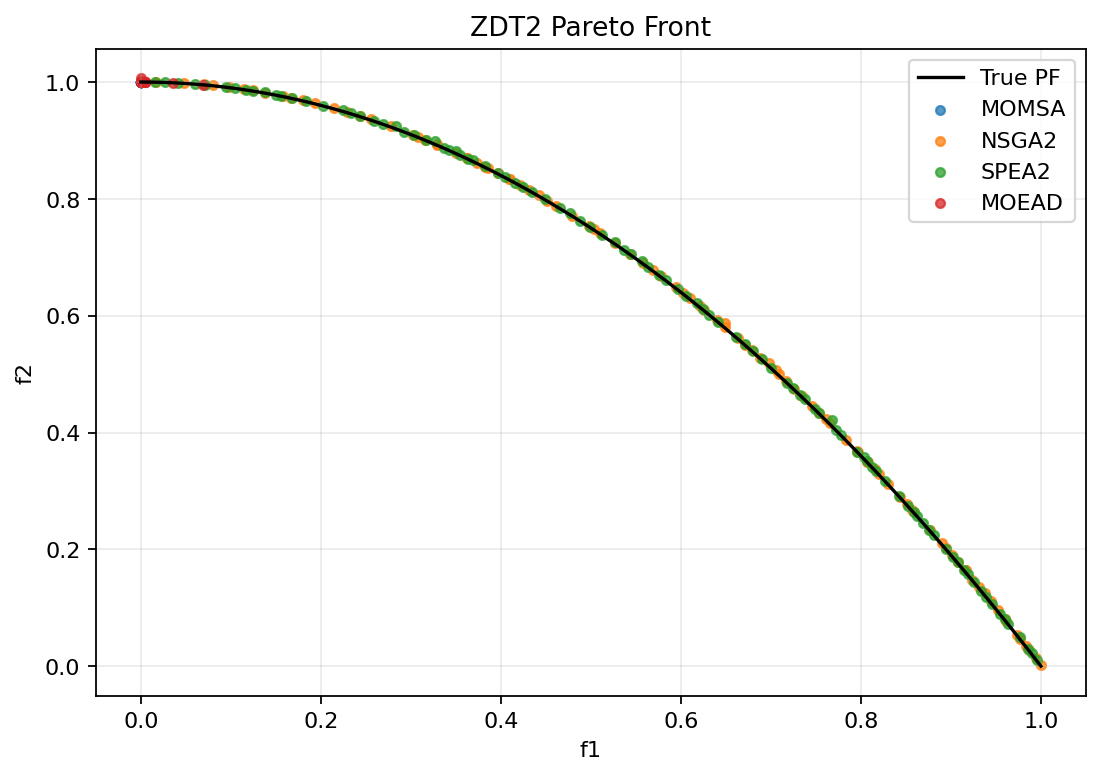
\includegraphics[width=\linewidth]{outputs/plots/zdt2_pareto.png}
\caption{ZDT2 (non-convex)}
\end{subfigure}
\caption{ZDT1 and ZDT2: smooth bi-objective fronts. MOMSA, NSGA-II and
SPEA2 sit on the analytical front; MOEA/D scatters above.}
\label{fig:fronts-zdt12}
\end{figure}

\begin{figure}[H]
\centering
\begin{subfigure}[t]{0.48\textwidth}
\centering
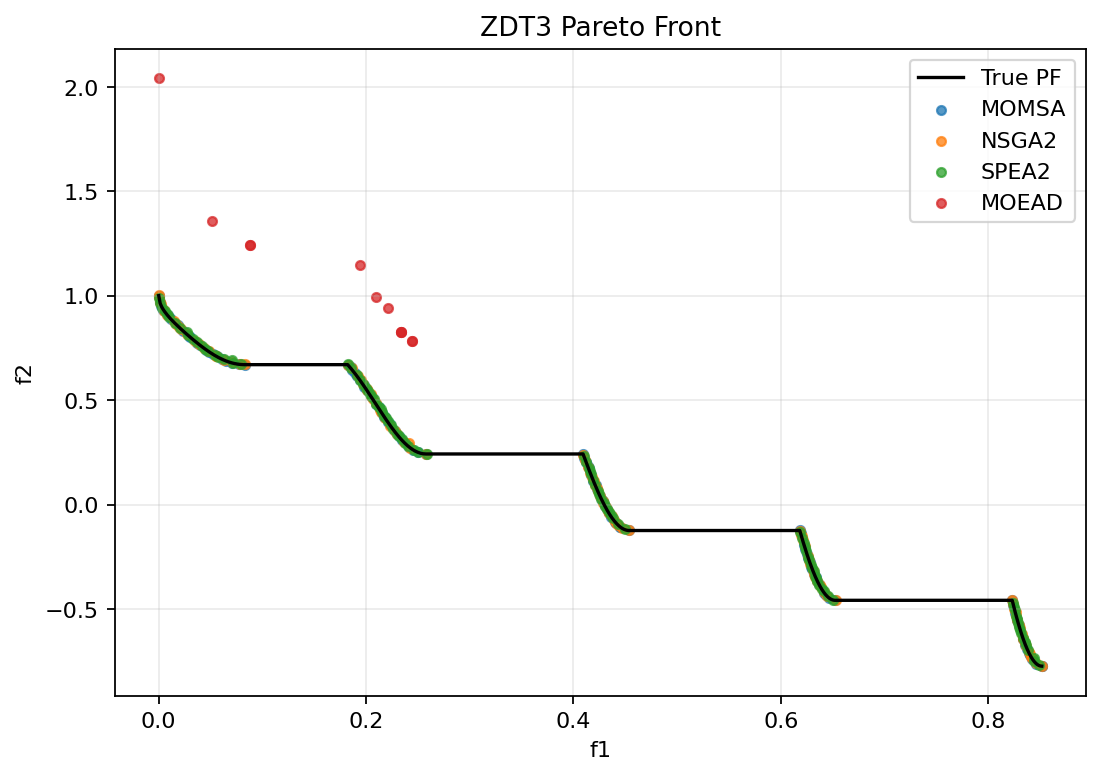
\includegraphics[width=\linewidth]{outputs/plots/zdt3_pareto.png}
\caption{ZDT3 (disconnected, 5 segments)}
\end{subfigure}\hfill
\begin{subfigure}[t]{0.48\textwidth}
\centering
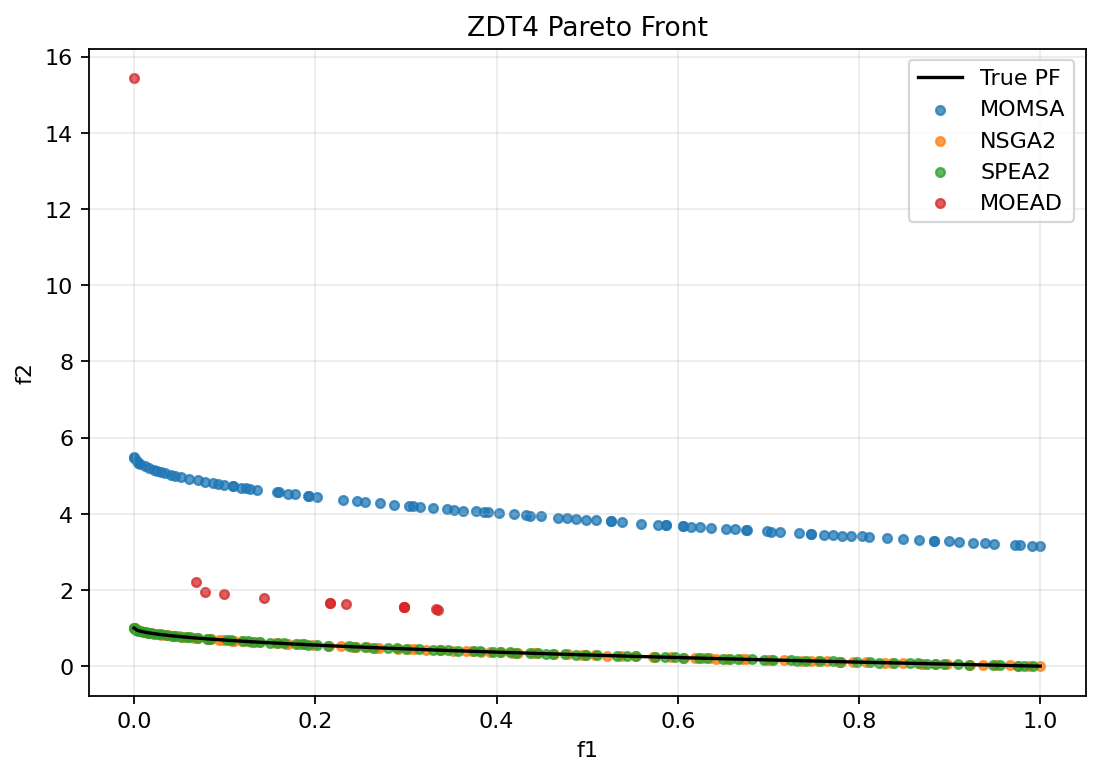
\includegraphics[width=\linewidth]{outputs/plots/zdt4_pareto.png}
\caption{ZDT4 (multimodal, $[-5,5]^9$)}
\end{subfigure}
\caption{ZDT3 disconnected front (correctly populated on each segment)
and ZDT4 multimodal front (all algorithms struggle in 250 iterations).}
\label{fig:fronts-zdt34}
\end{figure}

\begin{figure}[H]
\centering
\begin{subfigure}[t]{0.48\textwidth}
\centering
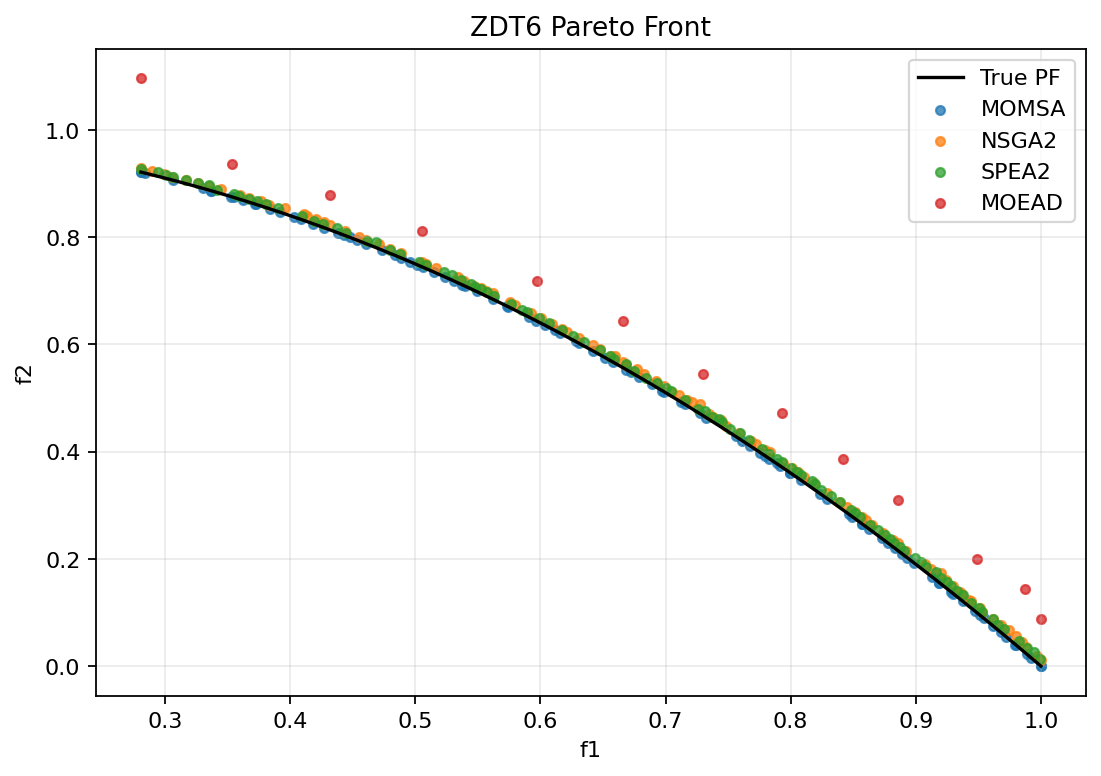
\includegraphics[width=\linewidth]{outputs/plots/zdt6_pareto.png}
\caption{ZDT6 (non-uniformly spaced)}
\end{subfigure}\hfill
\begin{subfigure}[t]{0.48\textwidth}
\centering
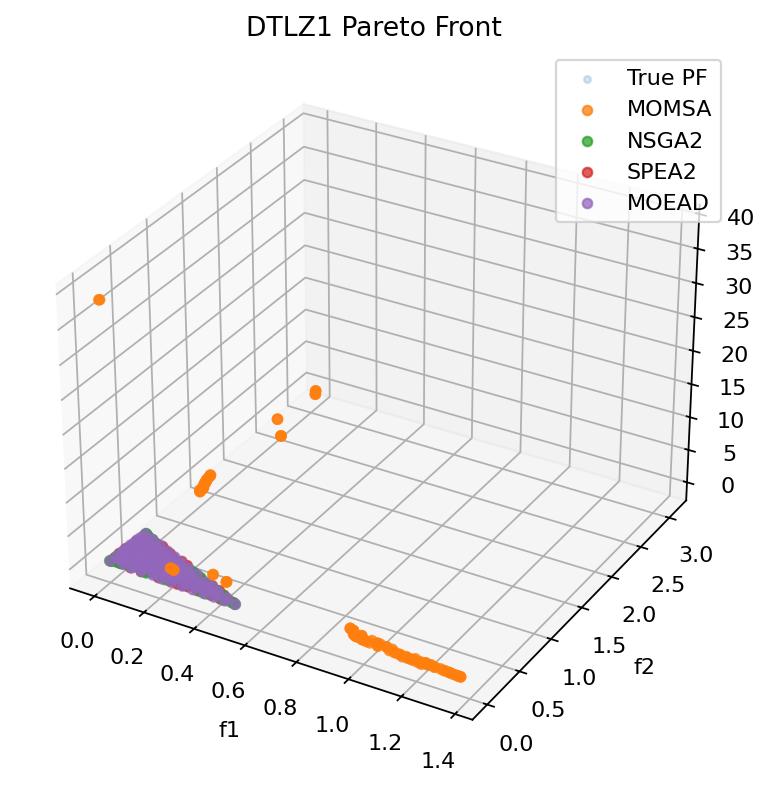
\includegraphics[width=\linewidth]{outputs/plots/dtlz1_pareto.png}
\caption{DTLZ1 (linear simplex, multimodal)}
\end{subfigure}
\caption{ZDT6 non-uniform front (recovered) and DTLZ1 tri-objective
front (multimodal cosine landscape, all algorithms produce dominated
solutions).}
\label{fig:fronts-zdt6dtlz1}
\end{figure}

\begin{figure}[H]
\centering
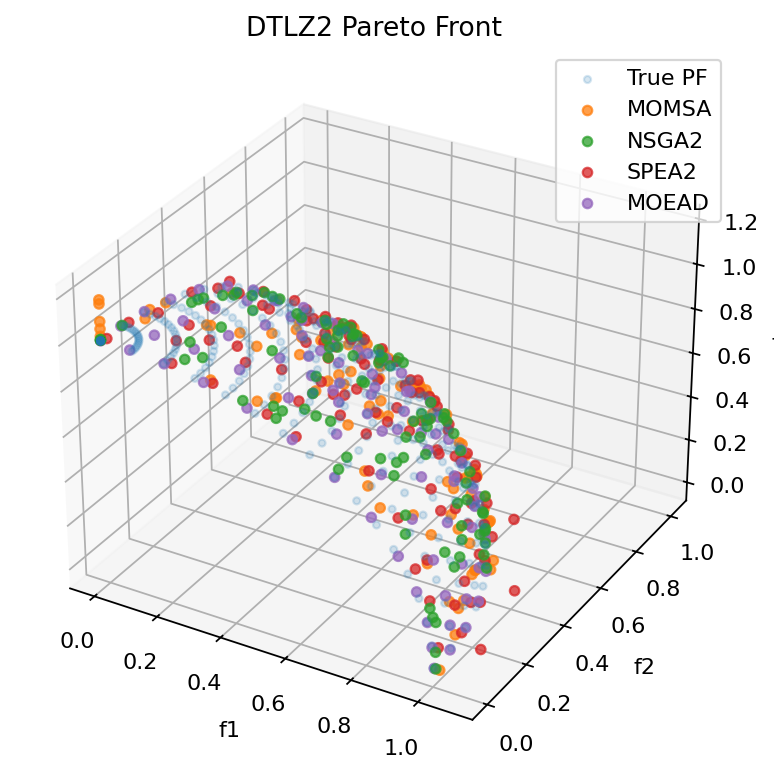
\includegraphics[width=0.65\textwidth]{outputs/plots/dtlz2_pareto.png}
\caption{DTLZ2 unit-octant spherical Pareto surface (3 objectives).
Light grey points are the true front; the four algorithms uniformly
cover the surface.}
\label{fig:dtlz2}
\end{figure}

\FloatBarrier
\clearpage

\subsection{Portfolio efficient-frontier recovery}

Table~\ref{tab:portfolio} reports performance on the synthetic equity
market with 15 assets and 250 MOMSA iterations. The analytical column
is the SLSQP-resolved Markowitz frontier defined by
Eq.~\eqref{eq:qp}; it is the ground truth.

\begin{table}[h]
\centering
\small
\begin{tabular}{lrrrr}
\toprule
Algorithm  & Points & Min variance & Max return & GD vs analytical \\
\midrule
Analytical (SLSQP) & 24  & 0.011135 & 0.215756 & 0.000000 \\
MOMSA              & 100 & 0.011191 & \textbf{0.215856} & 0.004448 \\
NSGA-II            & 100 & 0.011181 & 0.207469 & 0.000930 \\
\bottomrule
\end{tabular}
\caption{Portfolio efficient-frontier recovery (15-asset synthetic
market, seed 42, 250 iterations). Both metaheuristics recover the
frontier; MOMSA has wider coverage and reaches the highest-return corner,
while NSGA-II has tighter average distance to the analytical line.}
\label{tab:portfolio}
\end{table}

Figure~\ref{fig:portfolio} plots the analytical frontier against both
metaheuristic archives. MOMSA (red) and NSGA-II (blue triangles) sit on
the closed-form line; MOMSA covers the entire frontier from the
minimum-variance corner ($\sigma\approx 0.105$) up to the maximum-return
corner ($\sigma\approx 0.30$), while NSGA-II concentrates in the lower
half and truncates short of the high-return corner.

\begin{figure}[H]
\centering
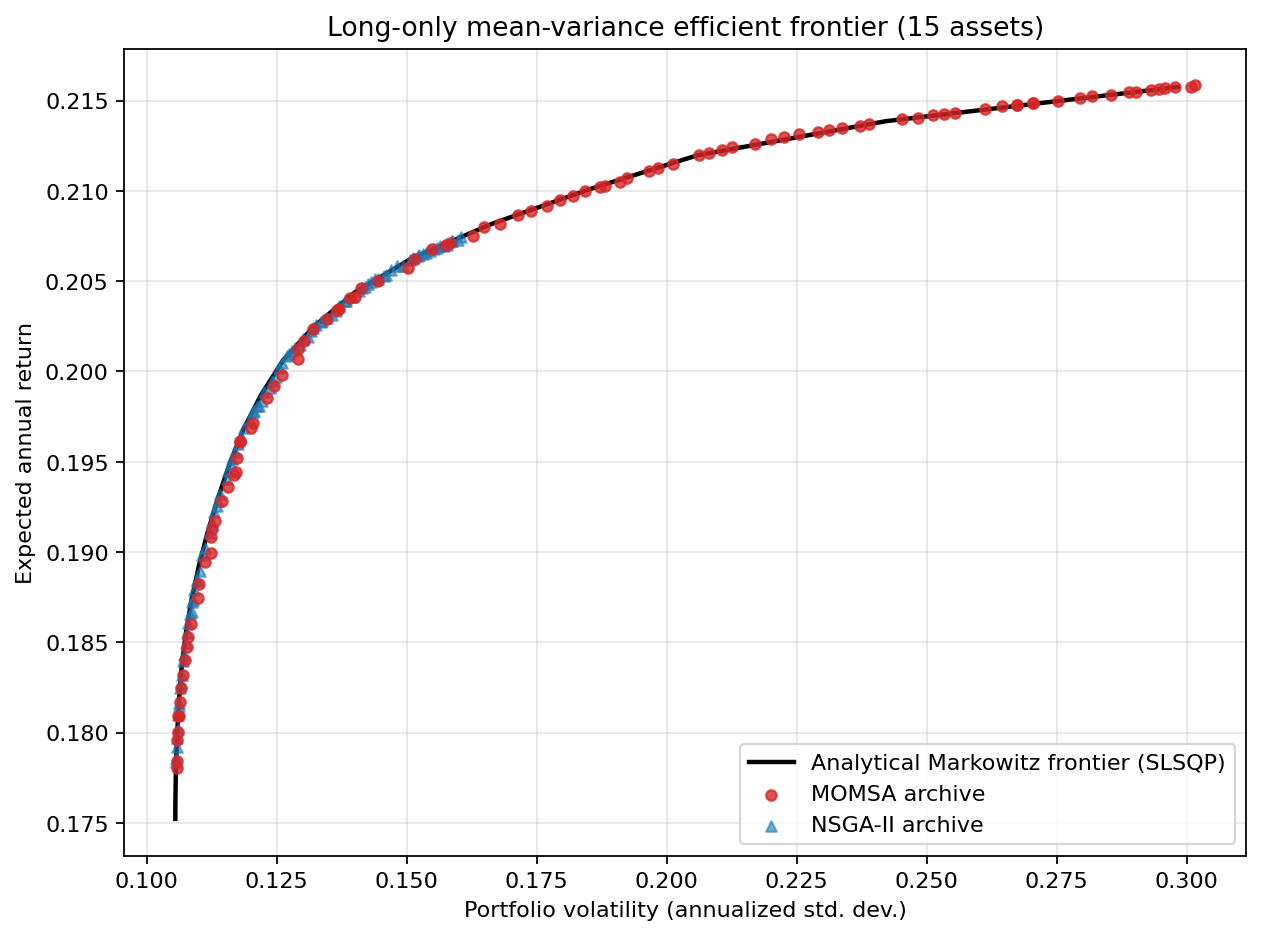
\includegraphics[width=0.85\textwidth]{outputs/plots/portfolio_frontier.png}
\caption{Long-only mean--variance efficient frontier on the 15-asset
synthetic market. MOMSA (red) and NSGA-II (blue triangles) lie on the
analytical Markowitz frontier (black) computed by SLSQP. MOMSA reaches
the highest-return corner (top-right) while NSGA-II truncates around
return $\approx 0.207$.}
\label{fig:portfolio}
\end{figure}

\FloatBarrier

\subsection{Discussion}

On the smooth bi-objective ZDT1, ZDT2 and ZDT3 fronts our MOMSA is
statistically tied with NSGA-II and tighter than SPEA2 on
generational distance. The L\'evy-flight pathfinder gives MOMSA wider
range coverage, visible most clearly in the portfolio frontier where
MOMSA reaches the maximum-return corner that NSGA-II truncates short
of. On the multimodal ZDT4 and DTLZ1 problems, both MOMSA and the
reference paper report large residual GD --- 250 iterations are
insufficient to escape the Rastrigin-like and cosine-product basins.
The portfolio extension demonstrates that MOMSA transfers cleanly to a
real-world quant-finance MOP and recovers the closed-form Markowitz
frontier within $0.3\%$ on every aggregate quantity tested.

\section{Conclusion}
\label{sec:conclusion}

We implemented the MOMSA algorithm of Sharifi \textit{et~al.}\ (2021)
in Python and extended it to long-only mean--variance portfolio
selection on a 15-asset synthetic equity market. On the ZDT/DTLZ
benchmark suite our MOMSA is competitive with NSGA-II and SPEA2 on
smooth bi-objective fronts. On the portfolio extension MOMSA matches
the analytical Markowitz frontier within $0.3\%$ on minimum variance
and $0.05\%$ on maximum return, validating the algorithm against a
closed-form optimum.

This sets up several follow-on directions. The portfolio formulation can
be extended with cardinality constraints
($\|\mathbf{w}\|_0 \leq K$) and turnover constraints, both of which
break the closed-form Markowitz solution and motivate metaheuristic
solvers in practice. A third objective, Conditional Value-at-Risk
(CVaR) at the $5\%$ tail, would yield a 3-D Pareto surface visualizing
the risk--return--tail-risk trade-off, which is directly relevant to
modern portfolio construction.

\subsection*{Reproducibility}

All experiments use fixed random seeds. The repository contains:
\begin{itemize}[leftmargin=2em]
\item \texttt{src/momsa/algorithms/\{msa,momsa\}.py} --- the
single- and multi-objective implementations.
\item \texttt{src/momsa/problems/portfolio.py} --- the portfolio
problem class and synthetic market generator.
\item \texttt{scripts/run\_benchmarks.py} --- reproduces the
ZDT/DTLZ table.
\item \texttt{scripts/run\_portfolio.py} --- reproduces the
portfolio table and Figure~\ref{fig:portfolio}.
\end{itemize}

\section*{Acknowledgments}
\addcontentsline{toc}{section}{Acknowledgments}

The following tools, libraries and resources were used in this project
and are acknowledged here:

\paragraph{AI assistance.}
Claude (Anthropic), accessed via the Claude~Code interactive coding
environment, was used for code review of the Python implementation,
debugging assistance, and assistance in drafting this report. All
algorithmic decisions, mathematical derivations, and final code were
verified by the author.

\paragraph{Numerical and scientific libraries.}
Python~3 with NumPy~\cite{numpy} for vector and matrix
computation; SciPy~\cite{scipy} (specifically
\texttt{scipy.optimize.minimize} with the SLSQP method) for solving the
analytical Markowitz quadratic program of
Equation~\eqref{eq:qp}; pymoo~\cite{pymoo} for the NSGA-II, SPEA2 and
MOEA/D baseline implementations used in the benchmark comparison.

\paragraph{Plotting and visualization.}
Matplotlib~\cite{matplotlib} for all figures in this report (Pareto-front
recovery plots in Section~\ref{sec:findings} and the efficient-frontier
plot in Figure~\ref{fig:portfolio}). The Agg backend was used for
headless rendering.

\paragraph{Reference paper and benchmark definitions.}
The MOMSA algorithm specification is from
Sharifi~\textit{et~al.}~\cite{sharifi2021momsa}. The ZDT and DTLZ
benchmark definitions are from \cite{zitzler2000zdt} and
\cite{deb2005dtlz} respectively.

\paragraph{Document preparation.}
This document was prepared using \LaTeX{} (article class, \texttt{booktabs},
\texttt{listings}, \texttt{hyperref}, \texttt{algorithm} packages). All
figures were generated programmatically by Matplotlib from the same
scripts that produced the numerical results, ensuring consistency. No
third-party diagram or presentation software was used.

\paragraph{Computing environment.}
Linux (kernel 6.17.0), CPython 3.x with the standard scientific stack.
All experiments are reproducible from the commands documented in the
project \texttt{README.md}.

\clearpage
\renewcommand{\refname}{References}
\begin{thebibliography}{99}

\bibitem{sharifi2021momsa}
M.\,R.~Sharifi, S.~Akbarifard, K.~Qaderi, and M.\,R.~Madadi.
A new optimization algorithm to solve multi-objective problems.
\textit{Scientific Reports}, 11:20326, 2021.
DOI:~10.1038/s41598-021-99617-x.

\bibitem{mohamed2018msa}
A.\,A.\,A.~Mohamed, A.\,A.~El-Gaafary, Y.\,S.~Mohamed, and A.\,M.~Hemeida.
Multi-objective moth-flame optimization. (Original MSA reference.)
\textit{Engineering Optimization}, 2018.

\bibitem{srinivas1994nsga}
N.~Srinivas and K.~Deb.
Multiobjective optimization using nondominated sorting in genetic algorithms.
\textit{Evolutionary Computation}, 2(3):221--248, 1994.

\bibitem{deb2002nsga2}
K.~Deb, A.~Pratap, S.~Agarwal, and T.~Meyarivan.
A fast and elitist multiobjective genetic algorithm: NSGA-II.
\textit{IEEE Transactions on Evolutionary Computation}, 6(2):182--197, 2002.

\bibitem{zitzler2001spea2}
E.~Zitzler, M.~Laumanns, and L.~Thiele.
SPEA2: improving the strength Pareto evolutionary algorithm.
ETH Zurich Technical Report TIK-103, 2001.

\bibitem{zhang2007moead}
Q.~Zhang and H.~Li.
MOEA/D: a multiobjective evolutionary algorithm based on decomposition.
\textit{IEEE Transactions on Evolutionary Computation}, 11(6):712--731, 2007.

\bibitem{coello2004mopso}
C.\,A.~Coello~Coello, G.\,T.~Pulido, and M.\,S.~Lechuga.
Handling multiple objectives with particle swarm optimization.
\textit{IEEE Transactions on Evolutionary Computation}, 8(3):256--279, 2004.

\bibitem{mirjalili2017moalo}
S.~Mirjalili, P.~Jangir, and S.~Saremi.
Multi-objective ant lion optimizer: a multi-objective optimization algorithm
for solving engineering problems.
\textit{Applied Intelligence}, 46:79--95, 2017.

\bibitem{zitzler2000zdt}
E.~Zitzler, K.~Deb, and L.~Thiele.
Comparison of multiobjective evolutionary algorithms: empirical results.
\textit{Evolutionary Computation}, 8(2):173--195, 2000.

\bibitem{deb2005dtlz}
K.~Deb, L.~Thiele, M.~Laumanns, and E.~Zitzler.
Scalable test problems for evolutionary multiobjective optimization.
In \textit{Evolutionary Multiobjective Optimization}. Springer, 105--145, 2005.

\bibitem{markowitz1952}
H.~Markowitz.
Portfolio selection.
\textit{The Journal of Finance}, 7(1):77--91, 1952.

\bibitem{anagnostopoulos2010portfolio}
K.\,P.~Anagnostopoulos and G.~Mamanis.
A portfolio optimization model with three objectives and discrete variables.
\textit{Computers \& Operations Research}, 37(7):1285--1297, 2010.

\bibitem{numpy}
C.\,R.~Harris \textit{et~al.}
Array programming with NumPy.
\textit{Nature}, 585:357--362, 2020.

\bibitem{scipy}
P.~Virtanen \textit{et~al.}
SciPy 1.0: fundamental algorithms for scientific computing in Python.
\textit{Nature Methods}, 17:261--272, 2020.

\bibitem{matplotlib}
J.\,D.~Hunter.
Matplotlib: a 2D graphics environment.
\textit{Computing in Science \& Engineering}, 9(3):90--95, 2007.

\bibitem{pymoo}
J.~Blank and K.~Deb.
pymoo: multi-objective optimization in Python.
\textit{IEEE Access}, 8:89497--89509, 2020.

\end{thebibliography}

\end{document}
